\documentclass[11pt,a4paper]{article}
\usepackage[T1]{fontenc}
\usepackage[utf8]{inputenc}
\usepackage{lmodern,microtype,amsmath,amssymb,graphicx,booktabs,longtable,array}
\usepackage[margin=24mm]{geometry}
\usepackage{listings,xcolor,fancyhdr}
\usepackage{url}
\usepackage[colorlinks=true,linkcolor=blue!45!black,citecolor=blue!45!black,urlcolor=blue!45!black]{hyperref}
\usepackage[numbers,sort&compress]{natbib}
\hypersetup{pdftitle={Indirect detection in MadDM: CosmiXsPPPC Earth fluxes and shared halo},pdfauthor={MadDM implementation documentation}}
\setlength{\emergencystretch}{3em}
\setlength{\parskip}{5pt}
\setlength{\parindent}{0pt}
\setlength{\headheight}{14pt}
\pagestyle{fancy}\fancyhf{}\lhead{MadDM indirect detection}\rhead{Implementation note: RAPIDD velocity profiles}\cfoot{\thepage}
\lstset{basicstyle=\ttfamily\small,breaklines=true,frame=single,columns=fullflexible,backgroundcolor=\color{black!3},keepspaces=true}
\newcommand{\sv}{\langle\sigma v\rangle}
\newcommand{\GeV}{\mathrm{GeV}}
\newcommand{\dd}{\mathrm{d}}
\newcommand{\pcbar}{\bar p}
\newcommand{\dbar}{\bar d}
\title{Indirect detection in MadDM:\\rates, spectra, likelihoods and antinucleus forecasts}
\author{Technical documentation of the supplied \texttt{rc/33/indirect} extension}
\date{5 November 2026 --- CosmiXsPPPC Earth fluxes and RAPIDD velocity profiles}
\begin{document}
\maketitle
\begin{abstract}
This note documents the calculations performed by the supplied MadDM plugin for dwarf-galaxy gamma rays, AMS-02 antiprotons, antideuteron forecasts and the Galactic-center excess. It follows the actual implementation from model parameters to saved numerical products. Particular attention is given to particle/antiparticle normalization, environment-dependent annihilation rates, the distinction between source yields and propagated fluxes, the shared Galactic density and velocity distribution, nuisance profiling and the meaning of reported limits. This is documentation of a particular code package and its statistical assumptions; it is not a new determination of transport parameters or a replacement for the experimental likelihoods. The LaTeX source, separate BibTeX file, example figures, regression tests and validation products accompany this PDF.
\end{abstract}
\tableofcontents
\clearpage

\section{Scope and the path from a model to an observable}
MadDM evaluates the annihilation processes of a chosen UFO model at a specified parameter point. Its original indirect-detection framework is described in Refs.~\cite{Ambrogi:2018jqj,Arina:2021gfn}. The present package extends the supplied \texttt{rc/33/indirect} snapshot with charged-cosmic-ray likelihoods, antideuteron event forecasts and a prompt Galactic-center spectral fit. The source snapshot identifies commit \texttt{3b3f8d1141c10c3a80bafb63d47ef47e721c48b8}. The extension considered here is for annihilation.

A run contains conceptually distinct calculations. Matrix elements determine partial annihilation rates. A source-spectrum calculation determines the number of particles produced per annihilation. Galactic transport converts charged-particle injection into an interstellar flux at the Sun. Solar modulation converts that local interstellar flux into a top-of-atmosphere flux. Experimental likelihoods or sensitivity prescriptions then map the prediction into limits, goodness-of-fit quantities or expected event counts. Confusing any two of these layers can introduce an extra density factor, duplicate propagation or an incorrect energy Jacobian.

The default charged-particle calculation selects an already propagated CosmiXsPPPC table. Consequently, the code does not apply another Galactic propagation operator to that table. It combines channel fluxes with the model branching fractions and rescales the result by the model rate and local density. The independently generated Pythia spectra remain source spectra. They can be used for the gamma-ray calculation and for inspecting model-dependent particle production, but they do not replace the tabulated antiproton or antideuteron flux used in the new charged-particle modules.

Every calculation writes into the ordinary \texttt{output/run\_XX} directory. A failed or unsupported calculation is explicitly marked unavailable. Negative sentinel values in summaries mean that an observable was not evaluated; they must never be read as an allowed model point.

\section{Model rates, branching fractions and velocities}
\subsection{Partial and total rates}
For a two-body final state $f$, write the partial annihilation rate as $\sv_f$. At fixed mass and velocity prescription, the total rate and branching fraction are
\begin{align}
\sv_{\mathrm{tot}} &= \sum_f \sv_f,\\
B_f &= \frac{\sv_f}{\sv_{\mathrm{tot}}}, \qquad \sum_f B_f=1.
\end{align}
Channels corresponding to the same physical pair are aggregated before forming $B_f$. The channel mapping uses final-state PDG identifiers, rather than relying on the spelling of generated process names. A nonzero unsupported channel is reported; it is not silently dropped followed by a renormalization of the supported branching fractions. Zero-rate channels do not change the mixture.

The propagated tables support 19 unpolarized channels:
\begin{align}
&e^+e^-,\ \mu^+\mu^-,\ \tau^+\tau^-,\ \nu_e\bar\nu_e,\ \nu_\mu\bar\nu_\mu,\ \nu_\tau\bar\nu_\tau,\\
&u\bar u,\ d\bar d,\ s\bar s,\ c\bar c,\ b\bar b,\ t\bar t,\\
&\gamma\gamma,\ gg,\ W^+W^-,\ ZZ,\ hh,\ \gamma Z,\ hZ.
\end{align}
The mixture assumes that the tabulated unpolarized spectra represent each generated pair. It does not reconstruct arbitrary polarization dependence from a UFO coupling choice. A new decay cascade or hidden-sector multi-body final state requires its own propagated charged-particle template; it is not equivalent to assigning its entire rate to a familiar two-body channel.

\subsection{Dwarf and Milky Way environments}
The continuum dwarf calculation uses \path|vave_indirect_cont|, with default
$2\times10^{-5}c$. By default the Galactic calculation uses the same Standard Halo Model as the RAPIDD nuclear recoil calculation. Its Galactic-frame distribution is isotropic,
\begin{equation}
 f[\mathbf v]\ \propto\
 \exp\!\left[-\frac{|\mathbf v|^2}{v_0^2}\right]
 \Theta\!\left[v_{\mathrm{esc}}-|\mathbf v|\right].
\end{equation}
The speeds $v_0$ and $v_{\mathrm{esc}}$ are \texttt{vMP} and \texttt{vescape},
with defaults of $238$ and $544\,\mathrm{km}\,\mathrm{s}^{-1}$. Recoil rates
boost this distribution into the laboratory frame. For annihilation the
laboratory boost cancels in $u=|\mathbf v_1-\mathbf v_2|$ for two independent
draws from $f$, and the partial rate is
\begin{equation}
 \sv_f=\int_0^{2v_{\mathrm{esc}}}p_{\mathrm{rel}}[u]\,
 \sigma_f[u]\,u\,\dd u.
\end{equation}
These rates are shared by the charged fluxes, the prompt GCE and Galactic
gamma lines. The common local SHM does not model a radial velocity
dependence. The dwarf velocity and J factors remain separate.

For the native SHM, MadDM derives $p_{\mathrm{rel}}$ from the overlap of
the two escape spheres and uses normalized Gauss--Legendre weights. Inclusive runs
evaluate the Fortran cross sections at each speed. Precise runs integrate
the generated partonic cross sections at the same energies, without
generating a separate unweighted event sample or shower. Both use incoming
speed $u/2$ in the pair centre-of-mass frame. Check convergence by increasing
\path|mw_shm_npts| for sharply velocity-dependent models. The optional
\texttt{mw\_velocity\_model=fixed} selects the legacy Galactic speed controls
with the default SHM only.

\subsection{Alternative RAPIDD velocity laws}
Set \path|halo_velocity_profile| to choose the underlying Galactic
distribution for both RAPIDD nuclear recoils and Milky Way annihilation.
The default \texttt{SHM} uses the native routines and requires no RAPIDD
installation for indirect detection. \path|SHM_numeric| integrates the
same distribution numerically. For \path|SHM_beta| and \texttt{Lisanti}
the phase-space factors inside the escape sphere are, respectively,
\begin{align}
 f_{\beta}[v]&\propto \exp[-v^2/v_0^2]-\beta\exp[-v_{\mathrm{esc}}^2/v_0^2],\\
 f_{\mathrm{Lisanti}}[v]&\propto
 \left[\exp[-v^2/[k v_0^2]]-\exp[-v_{\mathrm{esc}}^2/[k v_0^2]]\right]^k .
\end{align}
Both vanish outside the sphere and are separately normalized. The card
defaults are $\beta=1$ for \path|SHM_beta| and $k=1.5$ for \texttt{Lisanti}.
These profiles and their input conventions follow the velocity laws in
\href{https://github.com/cheekyparticle/RAPIDD_for_DM}{RAPIDD}.

The \path|SHM_wLMC| option adds a truncated Maxwellian centred on a
Galactic bulk velocity of magnitude $v_b$. For a local LMC fraction $f$,
the pair fractions are $[1-f]^2$, $2f[1-f]$ and $f^2$. The drift affects
smooth--LMC pairs. It cancels for LMC--LMC pairs. For recoils, MadDM uses
the RAPIDD reference laboratory angle plus an azimuth to fix the stream
direction in Galactic coordinates, then applies the time-dependent
laboratory boost. This direction does not affect the pair speed average.
The configurable parameters and the angle convention are documented in
\path|docs/HALO_VELOCITIES.md|.

MadDM evaluates the annual mean recoil integral for the selected velocity
law and passes its table to RAPIDD. The annihilation calculation uses the
same phase-space law to construct the pair distribution, including the LMC
cross pairs. For the numerical laws, the code integrates the angular
dependence for each pair of isotropic components in their respective rest
frames, then builds a normalized Gauss quadrature for the full relative
speed distribution. Dwarf velocity inputs remain separate.

\section{Run modes and what each comparison means}
\subsection{Fast or precise in sigmav mode}
In \texttt{indirect = sigmav}, source spectra are deliberately unnecessary for the per-channel experimental comparison. Each theoretical partial rate is compared with the corresponding BR$=1$ upper-limit curve. Dwarf curves come from \texttt{ExpData}; the original antiproton curves use QUAINT-MED, NFW and the default nuisance prescription. If a charged-table selection or likelihood setting differs, the pbar module profiles the relevant pure-channel template at the requested mass instead of reusing an incompatible stored bound.

A collection of pure-channel bounds is not a likelihood for the mixed final state. In particular, neither the minimum of those bounds nor their branching-weighted mean is a justified combined upper limit. The sigmav summary therefore reports channel comparisons without claiming a combined dwarf or pbar mixture limit. The Dbar forecast and GCE prompt fit can still be computed from a supported table mixture because those modules have their own spectral inputs.

\subsection{Flux modes}
When a prompt source spectrum is available, the dwarf likelihood can
evaluate the full mixture. Independently, \texttt{flux\_earth} writes
\path|CosmiXsPPPC_pbar_flux_earth.dat| and \path|CosmiXsPPPC_dbar_flux_earth.dat|.
These files give interstellar and top-of-atmosphere secondary, dark matter and
total differential fluxes at the model point. They use the configured
propagated tables and the fitted model-point solar potential when available,
or the \texttt{dbar\_phi} fallback. Charged fluxes remain available when the
antiproton likelihood and antideuteron forecasts are disabled. They require
no separate transport installation or source shower.

Integrated prompt photon and neutrino fluxes are still calculated when their
source spectra exist. Their display in the terminal and in
\texttt{MadDM\_results.txt} is suppressed. The positron flux calculation is
prepared for the analogous propagated and secondary spectra and will be
enabled once those inputs are available.

\section{One local density for recoils and Galactic annihilation}
\subsection{The public control}
The common card control is
\begin{lstlisting}
set rholocal 0.4
\end{lstlisting}
with units $\GeV\,\mathrm{cm}^{-3}$. This positive finite value is the common normalization for nuclear and electron recoil rates, capture, the pbar, Dbar and GCE calculations, and the Galactic gamma-line profile. It is validated before a run. It is not a free nuisance parameter in the pbar or GCE fits.

The old \texttt{pbar\_rho\_sun}, \texttt{gce\_rho\_sun} and gamma-line \texttt{rho\_sun} entries remain readable for old cards, but they do not override the common indirect normalization. Set \texttt{rholocal} explicitly when reproducing an old analysis. The legacy \texttt{rhoDM} field is synchronized with \texttt{rholocal} for the native recoil routines and RAPIDD. Recoil rates scale linearly with density; the published nucleon cross-section curves retain the experiments' reference halos. Dwarf J factors are properties of the dwarf galaxies and are not rescaled with the Milky Way density.

\subsection{Scaling laws and reference values}
The charged tables use $\rho_{\mathrm{ref}}=0.4\,\GeV\,\mathrm{cm}^{-3}$ and $\sv_{\mathrm{ref}}=3\times10^{-26}\,\mathrm{cm}^3\,\mathrm{s}^{-1}$. At fixed halo shape,
\begin{align}
\Phi_{\mathrm{DM}} &\propto \sv\,\rho_{\mathrm{local}}^2,\\
\sv_{\mathrm{UL}},\ \sv_{\mathrm{best}} &\propto \rho_{\mathrm{local}}^{-2},\\
N_{\dbar} &\propto \rho_{\mathrm{local}}^2.
\end{align}
Thus doubling \texttt{rholocal} multiplies the predicted model flux and event count by four, and divides the fitted annihilation rate and its normalization error by four. The minimum GCE chi-square is unchanged by this pure amplitude reparameterization.

The GCE geometry reference instead quotes $\rho_\odot=0.345\,\GeV\,\mathrm{cm}^{-3}$. Its dimensionless $\overline J$ is defined after dividing the density by its local value. Holding its shape fixed, using the common density is equivalent to multiplying the reference intensity by $[\rho_{\mathrm{local}}/0.345\,\GeV\,\mathrm{cm}^{-3}]^2$. This rescaling is applied once, through the explicit density squared in the GCE prefactor. No second rescaling of $\overline J$ is applied.

\section{Source normalization and particle/antiparticle conventions}
For a self-conjugate particle the usual annihilation source is
\begin{equation}
Q_a=\frac{1}{2}\frac{\rho^2}{m_\chi^2}\sv\sum_f B_f\frac{\dd N_{a,f}}{\dd E}.
\end{equation}
For a symmetric population of distinct particles and antiparticles, with $\rho$ denoting their total density, the corresponding pair-density factor is $1/4$ instead of $1/2$. The code uses the existing MadDM normalization factor $d_{\mathrm{MD}}=4$ for self-conjugate DM and $d_{\mathrm{MD}}=8$ for particle/antiparticle DM.

The charged-table control \texttt{pbar\_table\_convention} states the native source assumption. Its default is \texttt{self\_conjugate}; the alternative is \texttt{particle\_antiparticle}. The multiplier relative to the table is
\begin{equation}
f_{\mathrm{src}}=\frac{c_{\mathrm{native}}}{d_{\mathrm{MD}}/4},\qquad
c_{\mathrm{native}}=1\ \mathrm{or}\ 2.
\end{equation}
For the default native convention, a Dirac model receives half the self-conjugate flux at the same total density and rate. Dbar uses exactly the same source multiplier as pbar. This convention is explicit because the supplied propagated-table README states the benchmark rate and density but does not independently resolve every particle/antiparticle convention. Changing this control requires a consistent interpretation of both the UFO rate and the native tables.

\section{Data and table inventory}
\begin{longtable}{p{.23\linewidth}p{.69\linewidth}}
\toprule Input & Role and units\\\midrule\endhead
\texttt{ExpData/CR\_flux} & 54 propagated annihilation tables: 27 for each of pbar and Dbar. Three schemes, three transport sets and three halo profiles.\\
\texttt{ExpData/AMS02\_pbar} & The supplied AMS-02 rigidity-flux data and three secondary IS spectra, one per scheme.\\
\texttt{ExpData/AMS02\_dbar} & The three supplied secondary antideuteron IS spectra, used for reference curves.\\
\texttt{ExpData/GCE} & Supplied first-block GCE SED and compressed unpolarized CosmiXs prompt photon yields.\\
\texttt{Fermi\_Data} & Dwarf J factors and tabulated energy-bin likelihoods used by the combined dwarf analysis.\\
\texttt{ExpData} & Existing single-channel dwarf curves and the 19 precomputed QUAINT-MED/NFW pbar BR$=1$ curves.\\\bottomrule
\end{longtable}

The propagated charged tables are supplied with Ref.~\cite{Cirelli:2026CosmiXsPPPC}; the production spectra originate from CosmiXs~\cite{CosmiXsProduction}. The packaged annihilation grid contains 64 masses from 5 GeV to 100 TeV and a kinetic-energy grid from 0.1 to $10^5$ GeV. A table row contains the mass, $\log_{10}[K/\GeV]$ and 19 channel fluxes in $\GeV^{-1}\,\mathrm{m}^{-2}\,\mathrm{s}^{-1}\,\mathrm{sr}^{-1}$. For Dbar, $K$ is the total kinetic energy, not the kinetic energy per nucleon.

No dark-matter mass extrapolation is performed. Between adjacent masses the flux is interpolated linearly at fixed native energy. Energy interpolation is shape-preserving: positive intervals use a log-energy/log-flux PCHIP construction, and intervals touching a true zero retain zeros rather than extrapolating an arbitrarily small power law. Native values at or below $10^{-90}$ are interpreted as unpopulated-channel sentinels. A signal that is zero throughout the relevant domain yields an unavailable bound, not an enormous artificial numerical limit.

Source hashes and origin information are saved in the provenance JSON files. The full analysis does not download tables at run time. The selected propagation label, halo, density and input hashes are recorded with the numerical result.

\section{Propagation selection and secondary inputs}
The shared card controls are
\begin{lstlisting}
set cr_halo_profile NFW
set cr_propagation_scheme QUAINT
set cr_propagation_set MED
set pbar_secondary_file auto
\end{lstlisting}
The halo options are \texttt{NFW}, \texttt{Einasto} and \texttt{Burkert}; the schemes are \texttt{BIG}, \texttt{QUAINT} and \texttt{SLIM}; the sets are \texttt{MIN}, \texttt{MED} and \texttt{MAX}. These names refer to the supplied contemporary propagation tables, not the older transport benchmark numbers sometimes associated with the same MIN/MED/MAX labels. The transport framework is discussed in Ref.~\cite{Genolini2021}.

The DM primary flux uses the exact selected combination. Secondary pbar and Dbar inputs follow the scheme only. The six user-supplied zero-potential USINE spectra are stored without modifying their numerical values. For example, SLIM-MIN and SLIM-MAX share \texttt{secondary\_SLIM\_IS.txt}, while their primary DM fluxes use different propagated tables. This implements the requested approximation that residual secondary variations within a scheme are neglected.

The headers call the inputs TOA spectra, but the solar potential is zero. They can therefore be used as IS spectra and subsequently modulated. Their energy is $\GeV$/n and their differential flux is per $\GeV$/n. For pbar the nucleon number is one. The secondary Dbar input is already per nucleon and must not receive another factor of two in its flux normalization.

An explicit \texttt{pbar\_secondary\_file} overrides automatic pbar selection. It must contain two numeric columns with kinetic energy in GeV and flux in $\GeV^{-1}\,\mathrm{m}^{-2}\,\mathrm{s}^{-1}\,\mathrm{sr}^{-1}$. It is not a channel-dependent DM spectrum. Its path and hash enter the likelihood cache key, preventing a stale fit from being reused after a background file changes. Dbar reference curves continue to use the selected scheme's supplied input.

\section{Antiproton prediction and solar modulation}
\subsection{Interstellar mixture}
Let $\Phi^{\mathrm{tab}}_{\pcbar,f}$ be the selected propagated flux for one native channel. The model IS flux is
\begin{equation}
\Phi^{\mathrm{IS}}_{\pcbar,\mathrm{DM}}[K]=
\frac{\sv_{\mathrm{model}}}{\sv_{\mathrm{ref}}}
\left[\frac{\rho_{\mathrm{local}}}{\rho_{\mathrm{ref}}}\right]^2
f_{\mathrm{src}}\sum_f B_f\Phi^{\mathrm{tab}}_{\pcbar,f}[K].
\end{equation}
The mass dependence, spatial source distribution, $m_\chi^{-2}$ factor and Galactic propagation are already included in each native flux. They are not multiplied in again.

The secondary deformation is applied at interstellar kinetic energy:
\begin{equation}
\Phi^{\mathrm{IS}}_{\mathrm{sec}}[K]=
a\left[\frac{K}{K_0}\right]^\delta\Phi^{\mathrm{IS}}_{\mathrm{sec},0}[K],
\qquad a\in[0.8,1.2],\quad\delta\in[-0.1,0.1].
\end{equation}
The default pivot is $K_0=10$ GeV. The tilt is an energy-dependent multiplicative power law, not a remapping of the measured AMS energy grid. Its exponent is bounded in magnitude by 0.1, as requested. The normalization and tilt act on the secondary only.

\subsection{Force-field model and rigidity conversion}
For a species with total rest mass $m$ and charge magnitude $|Z|$, the force-field prescription used here is
\begin{align}
K_{\mathrm{IS}} &= K_{\mathrm{TOA}}+|Z|\phi,\\
\Phi^{\mathrm{TOA}}_K[K] & =
\frac{K[K+2m]}{[K+|Z|\phi][K+|Z|\phi+2m]}
\Phi^{\mathrm{IS}}_K[K+|Z|\phi].
\end{align}
For antiprotons $|Z|=1$ and $m=m_p$. The potential $\phi$ is fitted jointly with the secondary parameters; the default allowed range is 0--2 GV. It is an effective modulation potential for the supplied AMS data set, not a time-dependent heliospheric transport solution.

The supplied antiproton data are an AMS-02 rigidity-flux measurement; the experiment and its published results are described in Ref.~\cite{AMS:2021FirstSevenYears}. AMS data are differential in rigidity. At unit charge,
\begin{align}
K[R] &= \sqrt{R^2+m_p^2}-m_p,\\
\frac{\dd K}{\dd R} &= \frac{R}{\sqrt{R^2+m_p^2}},\\
\Phi_R[R] &= \Phi_K[K[R]]\frac{\dd K}{\dd R}.
\end{align}
Both primary and secondary components receive the same modulation and rigidity Jacobian at a given fit point. The native six-column data provide symmetric vertical errors and no nonzero horizontal bin widths. The comparison is made at the supplied rigidity abscissae; an unknown binning or covariance is not invented.

\section{Antiproton likelihood, upper limit and model test}
\subsection{Profile construction}
The conditional likelihood uses a diagonal chi-square,
\begin{equation}
\chi^2[s,a,\delta,\phi]=\sum_i
\frac{\left[\Phi_{\mathrm{sec},i}[a,\delta,\phi]+\Phi_{\mathrm{DM},i}[s,\phi]-D_i\right]^2}{\epsilon_i^2},
\qquad s=\sv\geq0.
\end{equation}
The supplied AMS vertical uncertainties $\epsilon_i$ are used as given. Their covariance and decomposition into correlated systematic components are not supplied. Consequently this is a reproducible diagonal-error analysis, conditional on the chosen secondary reference and nuisance bounds.

At each fixed $s$, the code minimizes over $a$, $\delta$ and $\phi$. The normalization is solved analytically at fixed tilt and potential, clipped to its hard interval; bounded numerical minimization handles the other two variables with multiple starts and derivative information. The scan includes the background-only point $s=0$, searches for the best nonnegative signal and brackets the upper crossing. A positive lower envelope over the continuous modulation interval supplies a large-rate ceiling. Root finding then refines the upper endpoint. Disconnected intervals are diagnosed and the largest upper crossing is reported.

The default one-sided asymptotic 95\% prescription is
\begin{align}
\chi^2_{\mathrm{prof}}[s_{95}]-\chi^2_{\mathrm{min}} &= 2.7055434541,\\
s_{\mathrm{best}} &= \mathop{\mathrm{arg\,min}}_{s\geq0}\chi^2_{\mathrm{prof}}[s].
\end{align}
This prescription is an explicit statistical convention of this package. It does not account for an additional covariance model or for marginalization over transport-table choices.

\subsection{Meaning of the three rates}
\begin{longtable}{p{.44\linewidth}p{.48\linewidth}}
\toprule Summary key & Meaning\\\midrule\endhead
\texttt{AMS02\_pbar\_sigmav\_UL95} & The profiled 95\% upper limit for the fixed model mixture.\\
\texttt{AMS02\_pbar\_sigmav\_best\_fit} & The rate preferred by pbar data after fitting secondary normalization, tilt and solar modulation.\\
\texttt{AMS02\_pbar\_sigmav\_model} & The theoretical total rate predicted by the chosen UFO couplings at the Galactic velocity prescription.\\\bottomrule
\end{longtable}
Their dimensions are all $\mathrm{cm}^3\,\mathrm{s}^{-1}$, but their meanings are different. The first two depend on the assumed fixed branching shape; the third is supplied by the model. The old numerical observable names remain as aliases in scan dictionaries for compatibility, but the human-readable summary prints the explicit names.

For the uploaded 100 GeV example, the old values $3.0691591\times10^{-26}$, $1.8252380\times10^{-26}$ and $1.0911031\times10^{-25}$ represent, respectively, the upper limit, best fit and coupling prediction. The coupling prediction is larger than the bound. A preferred nonzero pbar amplitude is not a claim that the selected full model, with its fixed couplings, is preferred by the data.

\subsection{The q values and relic-density rescaling}
The model-point statistic is
\begin{equation}
q_{\mathrm{upper}}[s]=
\begin{cases}
0,& s<s_{\mathrm{best}},\\
\max\{0,\chi^2_{\mathrm{prof}}[s]-\chi^2_{\mathrm{min}}\},&s\geq s_{\mathrm{best}}.
\end{cases}
\end{equation}
\texttt{AMS02\_pbar\_q\_upper\_model} evaluates it at $s=\sv_{\mathrm{model}}$. The \texttt{\_thermal} version evaluates it at $s=\xi^2\sv_{\mathrm{model}}$, where $\xi$ is the run's DM relic-density fraction. The two hypotheses are called AllDM and Thermal in the output. Their nuisance parameters are profiled separately. If $\xi=1$, their rates, statistics and decisions coincide exactly; this explains the equal values in the uploaded example.

A q value is dimensionless and is not a p-value. The code labels a model excluded when this one-sided statistic exceeds 2.7055434541. A rate below the best fit is not excluded by this upper-bound test even if it gives a worse two-sided fit. The full best-fit and model-point chi-square information remains available in JSON.

\section{Antiproton figures and saved nuisance configurations}
The flux file contains 15 named columns: rigidity, observed flux, error and three component columns for each of four configurations. Those configurations are the model-rate AllDM fit, the relic-rescaled model-rate fit, the free-amplitude best fit and the upper-limit fit. Each has its own secondary normalization, tilt and modulation potential.

The default figure displays the secondary, primary DM and total at the upper-limit configuration. It adds a separate primary DM curve at the theoretical model rate with that model point's fitted modulation. Thus a difference between the two DM curves need not be a pure constant amplitude ratio when their fitted solar potentials differ. The lower panel compares the upper-limit total with data using
\begin{equation}
\mathcal R_i=\frac{\Phi_{\mathrm{tot},i}-D_i}{\Phi_{\mathrm{tot},i}},\qquad
\epsilon_{\mathcal R,i}=\frac{\epsilon_i}{\Phi_{\mathrm{tot},i}}.
\end{equation}
The upper panel plots $R^3\Phi_R$ on logarithmic axes through at least 1 TV. The residual y axis remains linear, as explicitly requested for this signed quantity. This plotting choice does not alter a fit.

\begin{figure}[p]\centering
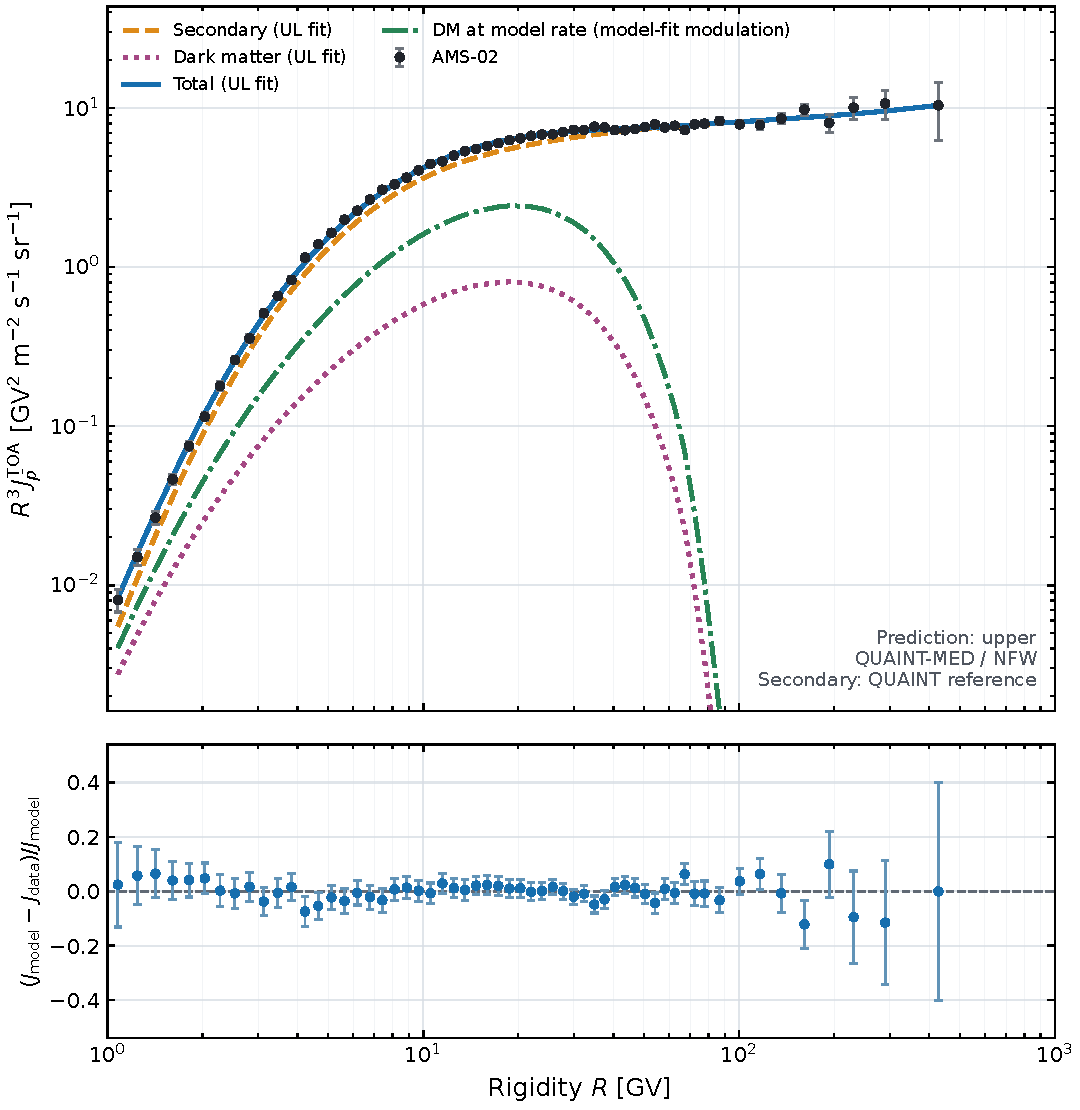
\includegraphics[width=.92\linewidth]{figures/AMS02_pbar_comparison.pdf}
\caption{Reanalysis of the uploaded 100 GeV run using its saved Galactic partial rates, the supplied QUAINT secondary spectrum and the common density of $0.4\,\GeV\,\mathrm{cm}^{-3}$. This is an actual table-based refit, rather than a new matrix-element calculation. The upper-limit nuisance configuration and theoretical-rate DM curve are distinct.}
\end{figure}

\section{Antideuteron fluxes, solar modulation and expected events}
\subsection{Energy per nucleon}
The propagated Dbar DM table is differential in total kinetic energy $K$, whereas the experimental windows use $T=K/A$ with $A=2$. The conversion is essential:
\begin{align}
K &= 2T, \qquad \frac{\dd K}{\dd T}=2,\\
\Phi_T[T] &= 2\Phi_K[2T].
\end{align}
Using total mass $m_d=1.875613$ GeV and $|Z|=1$, the primary TOA flux is
\begin{equation}
\Phi^{\mathrm{TOA}}_{T,\dbar}[T]=
2\frac{K[K+2m_d]}{[K+\phi][K+\phi+2m_d]}
\Phi^{\mathrm{IS}}_{K,\dbar}[K+\phi],\qquad K=2T.
\end{equation}
Equivalently, the solar shift in kinetic energy per nucleon is $\phi/2$. Applying a shift $\phi$ directly to $T$ would over-modulate Dbar. Omitting the prefactor two would undercount its differential flux.

The supplied secondary Dbar spectrum is already differential in $T$. Its modulation therefore uses the same momentum-squared ratio and shift $T\mapsto T+\phi/2$, without an extra energy Jacobian. The figure shows this separately as a secondary reference. Secondary events are not added to the DM signal event forecast.

\subsection{Choice of modulation potential}
When a successful full pbar model-point fit exists, Dbar uses its fitted AllDM potential. The Thermal Dbar forecast uses the corresponding relic-rescaled pbar model-point potential. It does not use the pbar upper-limit potential or the free-amplitude best-fit potential. In sigmav mode, or when no usable pbar flux fit exists, Dbar uses the explicit fixed \texttt{dbar\_phi}, default 0.7 GV. This choice is written to JSON and the console.

\subsection{Sensitivity-to-count prescription}
The adopted windows and flat sensitivities are
\begin{center}
\begin{tabular}{lrrr}\toprule
Experiment/window & $T_1$ & $T_2$ & sensitivity\\
 & \multicolumn{2}{c}{GeV/n} & $[\GeV/\mathrm n]^{-1}\,\mathrm m^{-2}\,\mathrm s^{-1}\,\mathrm{sr}^{-1}$\\\midrule
GAPS & 0.10 & 0.30 & $2\times10^{-6}$\\
AMS-02 low & 0.18 & 0.70 & $8\times10^{-7}$\\
AMS-02 high & 2.0 & 4.2 & $2\times10^{-7}$\\\bottomrule
\end{tabular}
\end{center}
They follow the user-specified two-event sensitivity prescription, also used in the antinucleus comparison of Ref.~\cite{DiMauro:2026SUEP}. In each window,
\begin{align}
\overline\Phi &= \frac{1}{T_2-T_1}\int_{T_1}^{T_2}\Phi^{\mathrm{TOA}}_{T,\dbar}[T]\,\dd T,\\
N_{\dbar} &= 2\frac{\overline\Phi}{\Phi_{\mathrm{sens}}},\\
N_{\mathrm{AMS}} &= N_{\mathrm{AMS,low}}+N_{\mathrm{AMS,high}}.
\end{align}
The integration uses the actual interpolated spectrum, with native table knots passed to adaptive quadrature. It is not a comparison of the peak flux with the threshold. A flat theory flux equal to the sensitivity produces exactly two expected events in that window, which is checked by regression tests.

These are approximate signal-count forecasts under the flat sensitivity prescription. No energy-dependent acceptance, efficiency matrix, energy dispersion or observation-time model is reconstructed. The factor two comes from the stated sensitivity definition and is not replaced by a different Poisson confidence-level count.

\begin{figure}[p]\centering
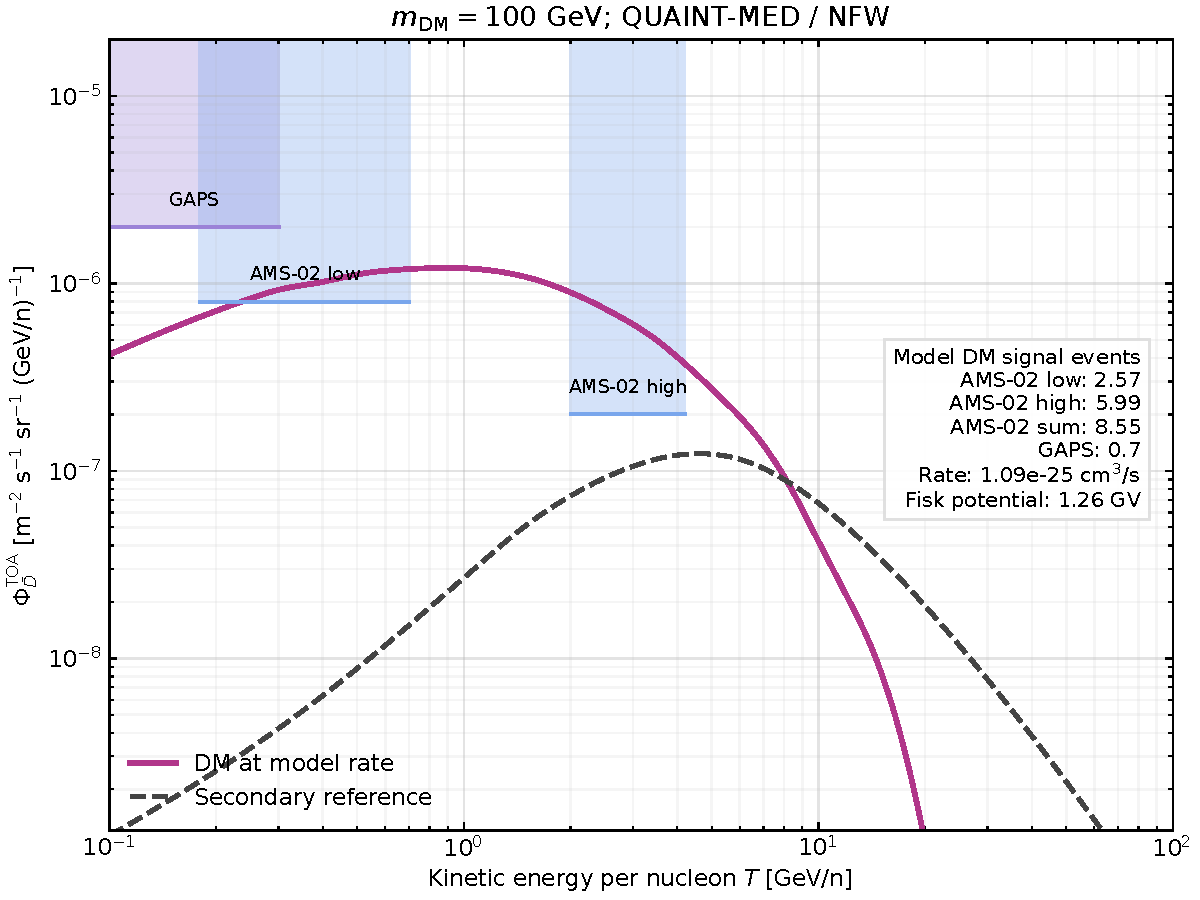
\includegraphics[width=.96\linewidth]{figures/AMS02_dbar_comparison.pdf}
\caption{Dbar prediction for the uploaded 100 GeV model mixture and rate. The sensitivity regions, signal counts, fitted solar potential and selected transport/halo setup are shown explicitly. The dashed secondary curve is a reference contribution and does not enter the quoted DM signal counts.}
\end{figure}

\section{Source antideuterons and the Argonne default}
Revision 9 sets both default Pythia cards and the Python card-class default to
\begin{lstlisting}
Main:methodDbar=4.0000000000e+00
\end{lstlisting}
Method 4 selects the existing Argonne Wigner-function implementation in \path|Templates/bin/main101.cc|, using the packaged \texttt{Argonne\_WF.txt}. Newly generated cards therefore choose Argonne by default. An already existing run card with an explicit different method is an intentional user setting; to switch it, edit \texttt{Cards/pythia8\_card.dat} or set the method in the card editor. Replacing defaults does not silently erase explicit old card choices.

The Pythia run calculates particle production spectra at the source. For Dbar these depend on its coalescence or wave-function prescription and the generated annihilation events. The flux at Earth used by the pbar/Dbar extension is evaluated from the separately bundled CosmiXsPPPC propagated tables. Switching the Pythia Dbar method changes its source-spectrum output; it does not regenerate the fixed CosmiXsPPPC Earth tables. A study intending to propagate the newly generated Argonne source spectrum requires a separate transport calculation and new template input.

The shower setup uses an absolute Les Houches event path and verifies event availability. End-of-file after processing available events is treated consistently, and an aborted/empty required gamma spectrum cannot be used to claim a dwarf limit. Unsupported optional spectra are diagnosed without turning their numerical artifacts into a valid flux. These compatibility checks belong to \texttt{indirect\_compat.py} and the source-spectrum reader.

\section{Dwarf-galaxy gamma-ray limits}
\subsection{Predicted bin energy flux}
The combined likelihood reads the packaged \texttt{Fermi\_Data/Jfactors.dat} and energy-bin likelihood grids, whose header identifies the 14-year dwarf analysis~\cite{McDaniel2024}. The branch selects 55 dwarfs and 26 energy bins. For dwarf $k$ and energy bin $i$, its prediction follows
\begin{equation}
F_{ik}[\sv]=\frac{\sv\,J_k}{2\pi d_{\mathrm{MD}}m_\chi^2}
\int_{E_{i,1}}^{E_{i,2}}E\frac{\dd N_\gamma}{\dd E}\,\dd E.
\end{equation}
Here $J_k$ is the dimensional, ROI-integrated dwarf J factor. The code's internal reference factor cancels against its stored relative J normalization; it does not make $J_k$ a Milky Way local-density quantity. The conversion from a source spectrum stored as $\dd N/\dd\log_{10}x$, with $x=E/m_\chi$, is
\begin{equation}
\frac{\dd N}{\dd E}=\frac{1}{E\ln10}\frac{\dd N}{\dd\log_{10}x}.
\end{equation}
The photon interpolator preserves zero intervals and the kinematic endpoint. Finite, ordered energy grids and nonnegative required photon yields are validated before evaluating a likelihood.

\subsection{Likelihood combination and confidence convention}
At each trial rate the module interpolates each published bin likelihood at the predicted bin energy flux and sums over energy bins and dwarfs. The original optional J-factor treatment is retained: when enabled, the likelihood is profiled over the packaged log-J uncertainties. Tabulated flux points outside the supplied likelihood range receive the branch's explicit low likelihood; they are not freely extrapolated.

The bounded solver in \texttt{fermi\_profile.py} scans the physical normalization and refines the upper crossing. It preserves the branch's dwarf confidence convention, namely the one-degree-of-freedom chi-square quantile at 95\%, $q=3.84145882$. This differs from the pbar one-sided threshold 2.7055434541. The package records this difference rather than silently changing a legacy Fermi convention.

\texttt{Fermi\_dSph\_limits.json} records the resulting combined limit, best likelihood and crossing diagnostics. In sigmav mode, individual \texttt{ExpData} curves are used instead. The exact source of a per-channel curve is the packaged curve, not a rerun of the 55-dwarf mixture likelihood. A common Milky Way density change leaves both kinds of dwarf bounds unchanged.

\section{Galactic-center excess: data, geometry and prompt spectrum}
\subsection{The first standard-analysis block}
The data file is the supplied SED associated with Ref.~\cite{GCEData2026}. The parser selects the first standard $40^\circ\times40^\circ$ ROI, with photon energy 0.5--1000 GeV and solid angle $\Delta\Omega=0.4775494185$ sr. There are 26 bins. The file contains energy reference and edges, central SED, statistical error, upper limit and lower/upper systematic envelopes.

The quoted SED is ROI-integrated in $\mathrm{MeV}\,\mathrm{cm}^{-2}\,\mathrm{s}^{-1}$. It is converted into a mean intensity by
\begin{equation}
Y_i=10^{-3}\frac{Y_{i,\mathrm{file}}}{\Delta\Omega},
\end{equation}
in $\GeV\,\mathrm{cm}^{-2}\,\mathrm{s}^{-1}\,\mathrm{sr}^{-1}$. The same conversion applies to the statistical errors and systematic bounds; energy columns receive the MeV-to-GeV factor only. Statistical errors are used in the figure. The requested fit uncertainties are derived from the systematic envelope.

Eleven rows contain detected central fluxes. Fifteen rows have the sentinel $-1$ for the central value and represent upper limits. Such rows are never used as negative flux measurements or replaced with zero-valued Gaussian observations. Their published upper limits and systematic upper envelopes are retained and checked separately. The minimum chi-square therefore describes only the 11 detected bins, with 10 degrees of freedom after fitting one amplitude.

\subsection{Dimensionless averaged geometrical factor}
The geometry follows Eqs.~37--39 and Table I of Ref.~\cite{GCEGeometry2025}. Define
\begin{equation}
\overline J=\frac{1}{\Delta\Omega}\int_{\mathrm{ROI}}\dd\Omega
\int_{\mathrm{los}}\frac{\dd\ell}{r_\odot}
\left[\frac{\rho[\ell,\Omega]}{\rho_\odot}\right]^2.
\end{equation}
The default is $\overline J=120$ and $r_\odot=8.122$ kpc. The prompt differential mean intensity is
\begin{equation}
\frac{\dd\Phi_\gamma}{\dd E}=\frac{r_\odot\rho_{\mathrm{local}}^2\overline J}{2\pi d_{\mathrm{MD}}m_\chi^2}
\sv\sum_f B_f\frac{\dd N_{\gamma,f}}{\dd E}.
\end{equation}
This is $1/[8\pi]$ for self-conjugate DM and $1/[16\pi]$ for a symmetric particle/antiparticle population. The local density is the common \texttt{rholocal}, while 0.345 GeV per cubic centimeter is saved as the original table's density reference. A dimensional integrated J factor must not be inserted into the dimensionless \texttt{gce\_jbar} setting, and the ROI solid angle must not divide the prediction a second time.

The GCE geometry is explicitly fixed unless its controls are changed. The charged-table halo setting does not replace $\overline J$ automatically, because it represents a separate requested GCE geometry. A consistent change of GCE halo shape requires the matching averaged factor. The common local normalization nevertheless applies to both.

\subsection{Spectral mixture and its limits}
The photon table is the official CosmiXs production table, restricted to 19 unpolarized channels and compressed losslessly in \texttt{CosmiXs\_gamma.npz}. Its original Git commit and SHA-256 are recorded in \texttt{ExpData/GCE/provenance.json}. For an in-grid mass, production yields are linearly interpolated in mass at fixed $x=E/m_\chi$. The mixture uses the model's Galactic branching fractions and converts $\dd N/\dd\log_{10}x$ into $\dd N/\dd E$.

This calculation is prompt-only. It does not include inverse-Compton scattering, bremsstrahlung, a new spatial transport solution for electrons or a change of GCE morphology with the final state. Equation 38 of the geometry reference concerns production and cascade spectra; it does not add another geometrical prefactor to a direct two-body spectrum. For unsupported multi-body models, an actual runtime photon spectrum is accepted in \texttt{fixed} mode only when it was produced at the same requested velocity and does not omit a separate positive line contribution. Otherwise the GCE fit is unavailable.

\section{GCE amplitude fit and visualization}
Let $P_i$ denote the predicted SED at $s_{\mathrm{ref}}=10^{-26}\,\mathrm{cm}^3\,\mathrm{s}^{-1}$ and let $A=s/s_{\mathrm{ref}}$. The mass and branching shape remain fixed. For detected bins, the split-normal chi-square is
\begin{align}
\chi^2[A]&=\sum_{i\in\mathrm{det}}\frac{[AP_i-Y_i]^2}{\sigma_i[A]^2},\\
\sigma_i[A]&=\begin{cases}
Y_i-L_i,&AP_i<Y_i,\\
U_i-Y_i,&AP_i\geq Y_i,
\end{cases}\qquad A\geq0.
\end{align}
Here $L_i$ and $U_i$ are the systematic envelope bounds. This treats the envelope as asymmetric diagonal one-sigma uncertainties. That is an explicit operational assumption, not a measurement of a bin covariance matrix. Statistical error bars shown on the figure are not added in quadrature a second time.

The piecewise quadratic objective is convex for valid bracketing errors. Its derivative is bracketed to find the physical minimum. The lower and upper amplitude errors solve $\chi^2[A]-\chi^2_{\mathrm{min}}=1$, respecting the nonnegative boundary. The code reports the best rate, separate lower and upper errors, the interval, chi-square and degrees of freedom. The optional symmetric error observable is their arithmetic mean; the asymmetric values remain the primary result.

For the censored rows the code records the best-fit SED, published statistical upper limit and systematic upper bound, and flags whether the best fit exceeds that systematic bound. These diagnostics must be inspected for a complete assessment. The fit is not a full likelihood including the 15 censored observations, and its 10-degree-of-freedom chi-square does not by itself establish compatibility with all high-energy limits. No chi-square p-value is assigned to the systematic-envelope fit.

The revised figure uses a grey filled systematic envelope through all 26 bins. Black detected points have statistical vertical errors and bin-width horizontal bars. Censored bins are shown with black arrows at the supplied published upper limits. The best-fit prompt model, its amplitude interval and the coupling-predicted curve are separate. The data band is not the same object as the blue model-amplitude interval.

\begin{figure}[p]\centering
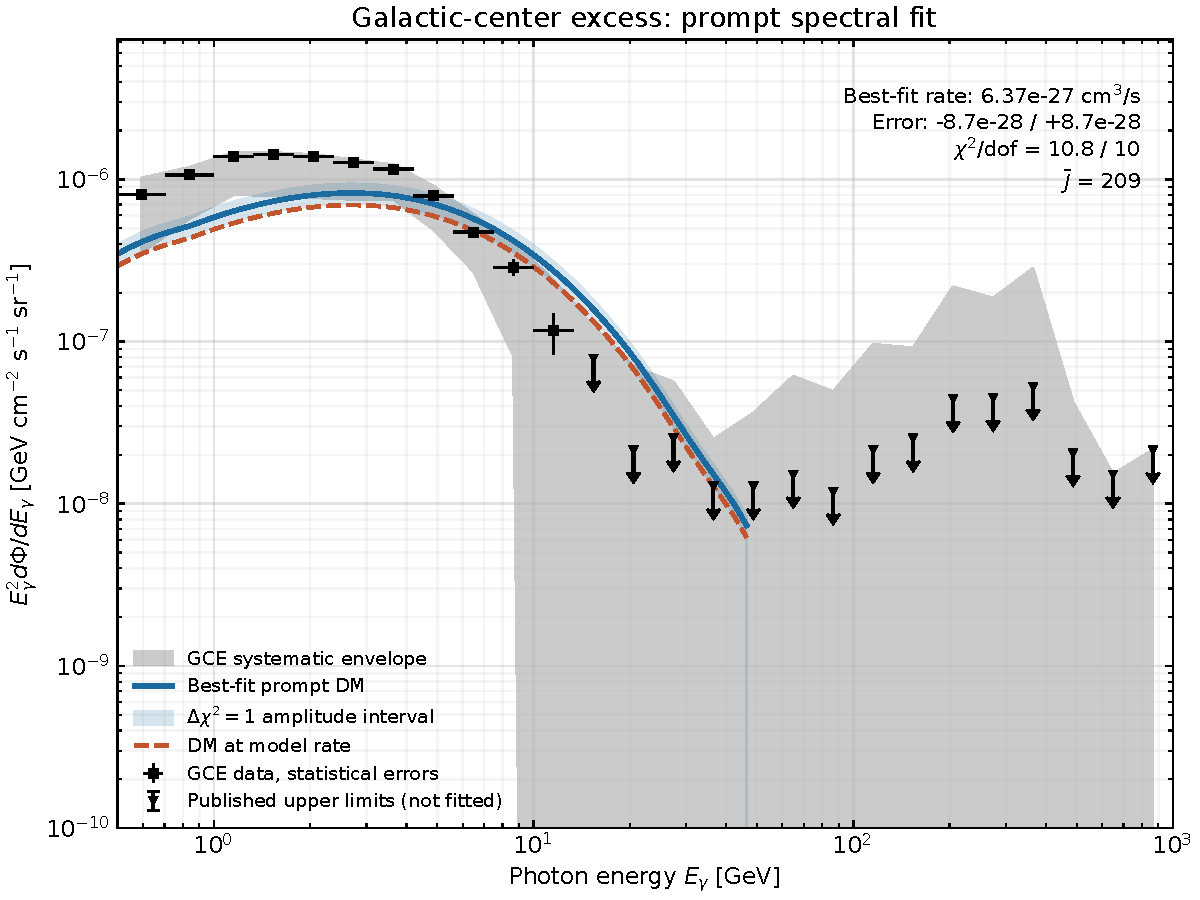
\includegraphics[width=.96\linewidth]{figures/GCE_example.pdf}
\caption{Historical GCE fit for the uploaded 50 GeV model mixture, recomputed with \texttt{rholocal=0.4}. The grey band is the supplied systematic envelope. Black points use the supplied statistical errors, while arrows identify published upper-limit bins that are not included as Gaussian detections. The blue band reflects only the fitted normalization uncertainty at fixed spectral shape.}
\end{figure}

\section{Software responsibilities and numerical safeguards}
\begin{longtable}{p{.32\linewidth}p{.60\linewidth}}
\toprule Module & Responsibility\\\midrule\endhead
\texttt{maddm\_run\_interface.py} & Card registration, run dispatch, build verification, rate collection, source-spectrum reading and results/scan integration.\\
\texttt{cr\_config.py} & Validated halo/scheme/set selection, matching secondary paths and common local density.\\
\texttt{halo\_model.py} & Shared card inputs, laboratory inverse-speed table and native rate-driver setup.\\
\path|velocity_profiles.py| & RAPIDD radial laws, boosted recoil integrals and the numerical pair quadrature.\\
\texttt{cr\_earth.py} & Charged flux files for the current model, including both IS and TOA components.\\
\texttt{pbar/core.py} & Native flux interpolation, force-field modulation, rigidity conversion, bounded nuisance profiles and pbar upper crossing.\\
\texttt{pbar\_interface.py} & PDG-channel mapping, branching mixtures, source convention, lookup/profile dispatch, result aliases and output products.\\
\texttt{dbar\_interface.py} & Total-energy/per-nucleon conversion, Dbar modulation, window integrals, event counts and diagnostics.\\
\texttt{gce\_interface.py} & SED parsing, prompt-yield mixture, common-density geometry, asymmetric amplitude fit and censored-bin diagnostics.\\
\texttt{fermi\_profile.py} & Vectorized bin-likelihood interpolation and bounded dwarf normalization solver.\\
\texttt{indirect\_compat.py} & MG5/Pythia compatibility, shower input preparation, spectrum validation and active-environment build helpers.\\
\texttt{signal\_plots.py} & GCE and Dbar PDF rendering from saved arrays.\\
\texttt{pbar\_plot.py} & Named-column pbar figure with upper-limit and model configurations.\\
\path|Templates/bin/main101.cc| & Event-level particle spectra and existing antideuteron formation prescriptions.\\\bottomrule
\end{longtable}

Caches use exact masses and branching fractions, selected table paths, source factors, local densities and likelihood configurations. The secondary-file hash is part of its cache identity. No rounded mass or approximate branching key is used to reuse an incompatible fit. A changed local density triggers the correct template and profile normalization. A changed theoretical rate at fixed shape reuses the shape-dependent upper bound but profiles the new model point.

Runtime products are written only for the current calculation status; obsolete flux files and figures are removed when the calculation cannot be evaluated. JSON excludes private NumPy arrays and disallows NaN. The numerical table outputs remain the authoritative input for regenerating a figure. Plotting failure is reported separately and does not turn a valid physics result into an allowed or excluded decision by itself.

The large warning output in the supplied log consists mainly of third-party DEBUG/INFO rendering records. MadGraph's coloring formatter can also mis-handle percent-format arguments in fontTools debug records, producing logging tracebacks. The plotting entry points now set Matplotlib and fontTools logger hierarchies to WARNING before importing/rendering. Actual warnings and errors are retained, as are unrelated MadDM debug messages. There is no global warning filter, no disabled exception handling and no change to a physics likelihood to quiet the output.

\section{Card settings and a reproducible run}
For a default Galactic analysis use
\begin{lstlisting}
indirect=flux_earth
set fast
set rholocal 0.4
set cr_halo_profile NFW
set cr_propagation_scheme QUAINT
set cr_propagation_set MED
set pbar_secondary_file auto
set pbar_limits True
set pbar_plot True
set dbar_events True
set dbar_plot True
set gce_fit True
set gce_plot True
\end{lstlisting}
For SLIM-MAX change the scheme and set only; the supplied SLIM secondary is selected automatically. For a channel-only comparison choose \texttt{indirect=sigmav} and either \texttt{set fast} or \texttt{set precise}. The common density and charged-table selection still apply.

\begin{longtable}{p{.39\linewidth}p{.15\linewidth}p{.38\linewidth}}
\toprule Control & Default & Interpretation\\\midrule\endhead
\texttt{rholocal} & 0.4 & Shared local density, GeV per cubic centimeter.\\
\texttt{cr\_halo\_profile} & NFW & Charged DM spatial-profile table.\\
\texttt{cr\_propagation\_scheme} & QUAINT & Charged transport scheme and secondary reference.\\
\texttt{cr\_propagation\_set} & MED & DM MIN/MED/MAX table.\\
\texttt{vMP}, \texttt{vescape} & 238, 544 & Shared SHM speeds in km/s.\\
\path|halo_velocity_profile| & SHM & Common RAPIDD recoil and Galactic annihilation law.\\
\path|mw_velocity_model| & shm & Average the selected law; fixed selects legacy speeds.\\
\path|mw_shm_npts| & 16 & Number of relative-speed integration nodes.\\
\path|vave_indirect_pbar| & 0.00075 & Galactic speed setting in units of $c$, used in fixed mode.\\
\texttt{pbar\_phi\_min/max} & 0 / 2 & Profile range in GV.\\
\texttt{pbar\_pivot} & 10 & Secondary tilt pivot in GeV.\\
\texttt{pbar\_rigidity\_min/max} & 0 / -1 & Data range; negative upper setting means all supplied data.\\
\texttt{dbar\_phi} & 0.7 & Fixed fallback potential in GV.\\
\texttt{gce\_jbar} & 120 & Dimensionless averaged GCE geometry.\\
\texttt{gce\_rsun\_kpc} & 8.122 & Geometry Solar radius.\\
\texttt{Main:methodDbar} & 4 & Argonne source prescription in the Pythia card.\\\bottomrule
\end{longtable}

Install the whole plugin directory as \texttt{PLUGIN/maddm}, restart MadDM and relaunch the generated project. Updating an unrelated Python environment does not update the plugin used by a running MG5 session. NumPy, SciPy and Matplotlib requirements are listed in \texttt{requirements-ams02.txt}. The charged Earth fluxes require no additional tables. Optional photon and neutrino source spectra have their own inputs.

For old generated projects the card reader supplies missing new defaults. If both local density entries are supplied, the common \texttt{rholocal} takes precedence. To recover the previous GCE-only normalization set \texttt{rholocal 0.345}; doing so now also changes the charged signals consistently. To change an old explicit source coalescence method, set \texttt{Main:methodDbar=4} in that project's Pythia card. Default migration is not a license to overwrite a user's explicit physics choices.

\section{Output dictionary and figure regeneration}
\begin{longtable}{p{.43\linewidth}p{.49\linewidth}}
\toprule Run product & Contents\\\midrule\endhead
\texttt{MadDM\_results.txt} & Dwarf/channel results, explicit pbar rates and q definitions, Dbar counts, GCE best fit/errors/chi-square.\\
\path|Halo_velocity.json| & Shared Galactic law, density, recoil and relative-speed table metadata.\\
\path|MW_relative_speed.dat| & Relative speeds and normalized weights used for the Galactic annihilation average.\\
\path|CosmiXsPPPC_*_flux_earth.dat| & IS and TOA charged flux components for the model and thermal rates.\\
\path|CosmiXsPPPC_flux_earth.json| & Earth flux input tables, unit conventions, solar potentials and status.\\
\texttt{Fermi\_dSph\_limits.json} & Combined dwarf likelihood diagnostics when a spectrum is available.\\
\texttt{AMS02\_pbar\_limits.json} & Full profile, fitted nuisance configurations, model tests, input hashes and assumptions.\\
\texttt{AMS02\_pbar\_fluxes.dat} & Model, Thermal, best-fit and upper-limit components at AMS rigidity points.\\
\texttt{AMS02\_pbar\_channel\_limits.dat} & Channel-only comparisons in sigmav mode.\\
\texttt{AMS02\_pbar\_comparison.pdf} & Upper-limit component figure with separate model-rate primary.\\
\texttt{AMS02\_dbar\_events.json/dat} & Window definitions, average signal fluxes, counts and modulation source.\\
\texttt{AMS02\_dbar\_fluxes.dat} & IS and TOA primary spectra for AllDM and Thermal.\\
\texttt{AMS02\_dbar\_secondary.dat} & Selected secondary TOA reference curve.\\
\texttt{AMS02\_dbar\_comparison.pdf} & Signal, reference secondary, sensitivities and event annotations.\\
\texttt{GCE\_fit.json/txt} & Prompt best fit, asymmetric interval, chi-square, geometry and upper-bin checks.\\
\texttt{GCE\_spectrum.dat} & Data/bin edges, systematic envelope, published upper limits, model/best prediction, fit mask and statistical errors.\\
\texttt{GCE\_prompt\_spectrum.dat} & Dense model, best, lower-interval and upper-interval prompt spectra.\\
\texttt{GCE\_fit.pdf} & Grey systematic envelope, black statistical data and fitted/model curves.\\\bottomrule
\end{longtable}

The stat-error column is appended to the GCE bin table so the original ten column positions remain unchanged. New files have eleven columns. The fit mask remains column ten in one-based counting; the new statistical-error column is column eleven. The plotting function also reads older ten-column results, but it does not fabricate missing statistical errors.

The following command regenerates available figures from a completed run without importing MadGraph:
\begin{lstlisting}
python examples/plot_run_products.py /path/to/output/run_XX
\end{lstlisting}
The self-contained pbar script accepts the named flux columns directly:
\begin{lstlisting}
python examples/plot_ams02_pbar_fluxes.py \
  /path/to/AMS02_pbar_fluxes.dat -o pbar.pdf
\end{lstlisting}
Its default is the upper-limit configuration. An explicit alternative prediction can be selected for diagnostic use. Figures are vector PDFs with embedded fonts and a 600-dpi save setting for any raster elements. Scientific flux panels use base-ten logarithmic axes; the signed pbar residual panel is linear.

\section{Validation strategy and interpretation limits}
The regression suite checks analytic constant-flux event counts, source-convention factors, density scaling, exact table nodes, absent signal channels, nondefault table selection, force-field Jacobians, nuisance constraints, upper crossings, scan serialization, required spectrum validation and the MG5 card contract. Additional revision-9 checks verify scheme-specific secondary selection, MIN/MED/MAX background invariance, shared density scaling across modules, explicit result names and the retention of real warning messages while rendering debug noise is omitted.

The supplied test run is reanalyzed from its saved Galactic partial rates to reproduce the pbar numerical values and new GCE figure. This checks the table/likelihood layer and does not pretend to be a fresh UFO matrix-element computation. Separate complete MG5 launches exercise the fast and precise dispatch paths; the validation directory distinguishes current checks from historical revision snapshots. Linux execution is used for the automated full-run validation; a native macOS run is not claimed here.

Several assumptions remain explicit. The AMS likelihood is diagonal. The secondary shape freedom is bounded, rather than a transport-parameter covariance fit. The GCE systematic envelope is represented by diagonal split-normal errors, and upper-limit bins are diagnostic checks rather than likelihood terms. The GCE is prompt-only. The charged tables describe the supplied two-body unpolarized spectra, and changing Pythia source coalescence does not regenerate them. The Dbar count estimate uses flat two-event sensitivities. These choices define what the numerical outputs mean and the scope in which they can be compared across models.

\appendix
\section{Density and unit checks useful for extending the code}
A future implementation should preserve four checks. First, a pure table channel at native mass, density and benchmark rate must reproduce its native IS flux. Second, a density change by a factor $c$ must multiply every Galactic model flux by $c^2$, while dwarf predictions remain fixed. Third, conversion from Dbar total kinetic energy to per-nucleon energy must preserve the integrated number flux:
\begin{equation}
\int_{T_1}^{T_2}\Phi_T[T]\,\dd T
=\int_{2T_1}^{2T_2}\Phi_K[K]\,\dd K.
\end{equation}
Fourth, converting ROI-integrated GCE data into a mean intensity must not be accompanied by an additional division of a prediction already normalized with $\overline J$.

In a new propagated template, specify whether it is differential in total energy, kinetic energy or kinetic energy per nucleon; state the area unit, solar potential, native density, rate and particle/antiparticle convention. A file named ``spectrum'' is not sufficient evidence that it is a source yield. The likelihood accepts a local IS flux template, whose density and annihilation prefactors are already present. When these conventions are explicit, the pbar and Dbar modules can share the same mixture and normalization without repeating a Galactic transport computation.

\section{Building this note}
The document is kept as editable LaTeX and a separate BibTeX file:
\begin{lstlisting}
cd docs
pdflatex -halt-on-error indirect_detection_notes.tex
bibtex indirect_detection_notes
pdflatex -halt-on-error indirect_detection_notes.tex
pdflatex -halt-on-error indirect_detection_notes.tex
\end{lstlisting}
The three figure PDFs are included under \texttt{docs/figures}. They come from the actual table-based reanalysis of the supplied run. Recompiling the note does not execute a physics fit, modify a run card or change a model result.

\bibliographystyle{unsrtnat}
\bibliography{references}
\end{document}
